\documentclass{beamer}
\usetheme{Madrid}

\title{Error bounds for elliptic PDEs}
\author{Daniel Gallo}
\institute{University of Bergen}
\date{25 May 2021}

\usepackage{amsmath}
\usepackage{amssymb}
\usepackage{mathtools}
\usepackage{bm}
\usepackage{cancel}
\def\R{\mathbb{R}}
\newcommand{\norm}[1]{\left\lVert#1\right\rVert}
\DeclarePairedDelimiter\set\{\}


\begin{document}
    \begin{frame}
        \titlepage
    \end{frame}

    \begin{frame}{The heat equation}
        The \textbf{temperature} depends on \textbf{position} and \textbf{time}
        \begin{align*}
            u \colon \R^{n + 1} &\to \R \\
            (x_1, \dots, x_n, t) &\mapsto u(x_1, \dots, x_n, t)
        \end{align*}
        The \textbf{temperature} satisfies the \textbf{heat equation}
        \begin{equation*}
            u_t = \Delta u
        \end{equation*}
    \end{frame}

    \begin{frame}{The steady state heat equation}
        We assume that $u_t = 0$
        \begin{itemize}
            \item For the \textbf{homogenius} case, we have \textbf{Laplace's equation}
            \begin{equation*}
                \Delta u = 0
            \end{equation*}
            \item For the \textbf{inhomogenius} case (there is a heat source), we use \textbf{Poisson's equation}
            \begin{equation*}
                \-k \Delta u = f \implies
                \begin{cases}
                    \nabla \cdot \bm{q} = f \\
                    \bm{q} = -k \nabla u
                \end{cases}
            \end{equation*}
            \begin{itemize}
                \item $f$ is the \textbf{heat-flux density} of the source
                \item $k$ is the \textbf{thermal conductivity}
                \item $\bm{q}$ is the \textbf{flux} TODO
            \end{itemize}
        \end{itemize}
    \end{frame}

    \begin{frame}{Elliptic PDEs}
        Second-order linear PDEs can be written as
        \begin{equation*}
            Au_{xx} + 2Bu_{xy} + Cu_{yy} + Du_x + Eu_y + Fu + G = 0
        \end{equation*}
        In our case,
        \begin{equation*}
            -ku_{xx} -ku_{yy} - f = 0
        \end{equation*}
        Since $B^2 - AC = -k^2 < 0$, we say that our PDE is \textbf{elliptic}
    \end{frame}

    \begin{frame}{The numerical method}
        A little bit of notation
        \begin{itemize}
            \item The approximation of $u$ will be called $v$
            \item The approximation of $\bm{q}$ will be called $\bm{r}$
        \end{itemize}
        Two main steps
        \begin{enumerate}
            \item Discretization
            \item Solve a linear system of equations
            \item Interpolation
        \end{enumerate}
    \end{frame}

    \begin{frame}{The numerical method: discretization}
        \begin{columns}
            \column{0.45\textwidth}
            \begin{itemize}
                \item f at nodes
                \begin{align*}
                    f_1 = f(0, 0) \\
                    f_5 = f(1, 0) \\
                \end{align*}
                \item Flux based on finite difference
                \begin{itemize}
                    \item Recall that
                    \begin{equation*}
                        \bm{q} = -k \nabla u
                    \end{equation*}
                    \item Flux at edge 6
                    \begin{equation*}
                        r_6 = -k \frac{v_8 - v_7}{\Delta x}
                    \end{equation*}
                \end{itemize} 
            \end{itemize}
            \column{0.55\textwidth}
            \begin{figure}
                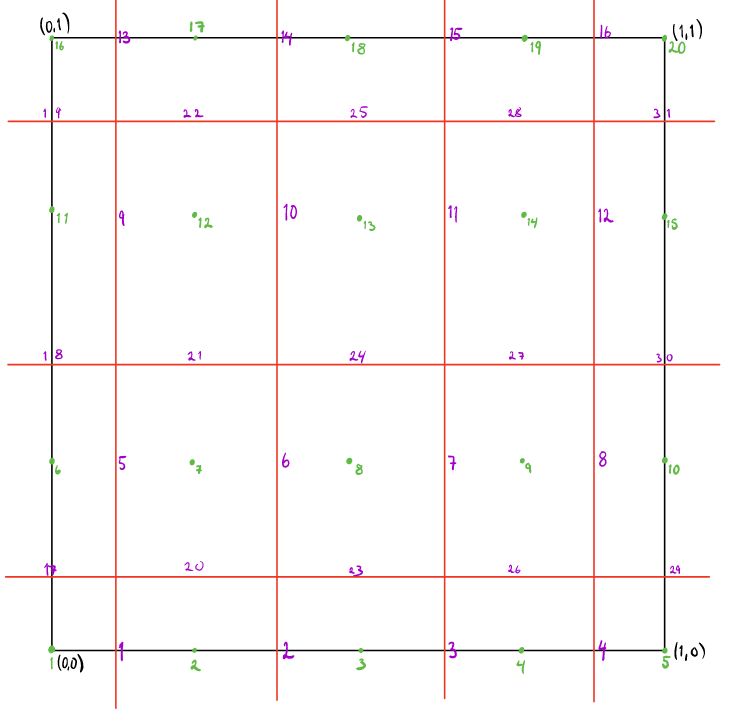
\includegraphics[scale=0.24]{grid.png}
            \end{figure}
        \end{columns}
    \end{frame}

    \begin{frame}{The numerical method: the divergence}
        Recall that
        \begin{equation*}
            \Delta \cdot \bm{q} = f
        \end{equation*}
        By Green's Theorem, in each cell $w$
        \begin{equation*}
            \oint_{\delta w} \bm{q} \cdot \hat{\bm{n}} ds = \iint_w \Delta \cdot \bm{q} dA = \iint_w f dA
        \end{equation*}
        Dividing by $\Delta x \Delta y$, we can approximate the double integral by $f$.
        \begin{equation*}
            \frac{1}{\Delta x \Delta y} (r_7 \Delta y + r_{24} \Delta x - r_6 \Delta y - r_{23}\Delta x) = f_8
        \end{equation*}
        \begin{figure}
            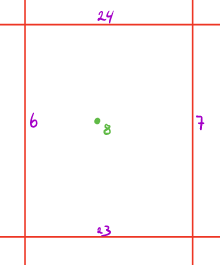
\includegraphics[scale=0.24]{cell.png}
        \end{figure}
    \end{frame}

    \begin{frame}{The numerical method: the system}
        We just have to solve for $v$
        \begin{equation*}
            D \cdot \underbrace{(-K \odot G) 
            \begin{bmatrix}
                v_1 \\
                v_2 \\
                v_3 \\
                \vdots \\
            \end{bmatrix}}_{\bm{r}}
            = 
            \begin{bmatrix}
                f_1 \\
                f_2 \\
                f_3 \\
                \vdots
            \end{bmatrix}
        \end{equation*}
    \end{frame}

    \begin{frame}{The numerical method: interpolation}
        \begin{columns}
            \column{0.6\textwidth}
                \begin{itemize}
                    \item Temperature $v$ at $P$
                    \begin{itemize}
                        \item B. inter. between $v_7$, $v_8$, $v_{13}$ and $v_{12}$
                        \begin{equation*}
                            v(x, y) = a_1 + a_2 x + a_3 y + a_4 xy
                        \end{equation*}
                    \end{itemize}
                    \item Flux $\bm{r} = (r_1, r_2)$ at $Q$
                    \begin{itemize}
                        \item For $r_1$: inter. between $r_5$ and $r_6$
                        \item For $r_2$: inter. between $r_{20}$ and $r_{21}$ 
                        \begin{equation*}
                            \bm{r}(x, y) = \begin{bmatrix}
                                b_1 + b_2 x \\
                                b_3 + b_4 y
                            \end{bmatrix}
                        \end{equation*}
                    \end{itemize}
                    
                \end{itemize}
            
            \column{0.4\textwidth}
                \begin{figure}
                    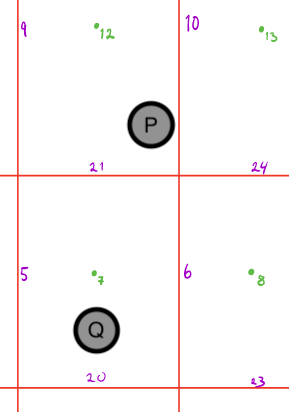
\includegraphics[scale=0.3]{interpolation.png}
                \end{figure}
        \end{columns}
    \end{frame}

    \begin{frame}{What about the boundary?}
    \begin{columns}
        \column{0.65\textwidth}
        \begin{itemize}
            \item \textbf{Edge} cells: Green's Theorem
            \begin{equation*}
                \frac{1}{\Delta x \Delta y} \left(r_5 \Delta y + \cancelto{0}{r_{18} \frac{\Delta x}{2}} - r_l \Delta y - \cancelto{0}{r_{17} \frac{\Delta x}{2}}\right) = f_6
            \end{equation*}
            \item \textbf{Corner} cells: 
            \begin{itemize}
                \item Same trick if signs match
                \item Force $\nabla \cdot \bm{r} = f$ if $f$ is constant
                \item Force $\bm{r}$ to be zero where it is zero
            \end{itemize}
        \end{itemize}
        \column{0.35\textwidth}
        \begin{figure}
            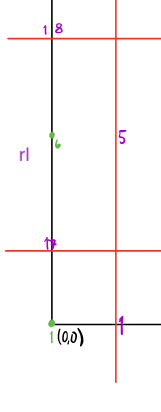
\includegraphics[scale=0.3]{edge.png}
        \end{figure}
    \end{columns}
        
    \end{frame}

    \begin{frame}{Error bounds}
        \begin{itemize}
            \item We want to measure how far our solution $v$ is from the real solution $u$
            \begin{equation*}
                \norm{e} = \norm{u - v}
            \end{equation*}
            \item The \textbf{energy norm} $\norm{\sqrt{k}\nabla e}$ is easier to bound
            \begin{equation*}
                \norm{\sqrt{k}\nabla e} \leq \norm{\frac{1}{\sqrt{k}} (\bm{r} + k\nabla v)} + C_{\Omega, k} \norm{f - \nabla \cdot \bm{r}} \equiv M(v, \bm{r}, f)
            \end{equation*}
        \end{itemize}
    \end{frame}

    \begin{frame}{Poincarè-Friedrichs constant}
        \begin{itemize}
            \item The \textbf{Poincarè-Friedrichs constant} is defined as follows
            \begin{equation*}
                C_{\Omega, k} = \sup\set*{\frac{\norm{e}}{\norm{\sqrt{k}\nabla e}}}
            \end{equation*}
            \item Thus, we can obtain a bound for the actual error!
            \begin{equation*}
                \norm{u - v} \leq C_{\Omega, k} \norm{\sqrt{k}\nabla e} \leq C_{\Omega, k}M(v, \bm{r}, f)
            \end{equation*}
        \end{itemize}
    \end{frame}

    \begin{frame}{Poincarè-Friedrichs constant}
        \begin{itemize}
            \item For \textbf{homogenius} $k$,
            \begin{equation*}
                C_{[0, 1]^2, k} = \frac{1}{\sqrt{2 k} \pi}    
            \end{equation*}
            \item For \textbf{arbitrary} $k$ we have to use the eigs function TODO
        \end{itemize}
    \end{frame}

    \begin{frame}{Errors}
        \begin{itemize}
            \item Error
            \begin{equation*}
                \norm{u - v} \leq C_{\Omega, k} M(v, \bm{r}, f)
            \end{equation*}
            \item Energy error
            \begin{equation*}
                \norm{\sqrt{k} \nabla e} \leq M(v, \bm{r}, f) ,\quad \quad I = \frac{M(v, \bm{r}, f)}{\norm{\sqrt{k} \nabla e}}
            \end{equation*}
            \item Star error
            \begin{equation*}
                M(v, \bm{r}, f) \leq \norm{(e_v, e_{\bm{r}})}_\star \leq 3 M(v, \bm{r}, f)
            \end{equation*}
            \begin{equation*}
                \norm{(e_v, e_{\bm{r}})}_\star = \norm{\sqrt{k} \nabla e} + \norm{\frac{\bm{q} - \bm{r}}{\sqrt{k}}} + C_{\Omega, k} \norm{\nabla \cdot (\bm{q} - \bm{r})}
            \end{equation*}
        \end{itemize}
    \end{frame}

    \begin{frame}{Error comparison}
        \begin{figure}
            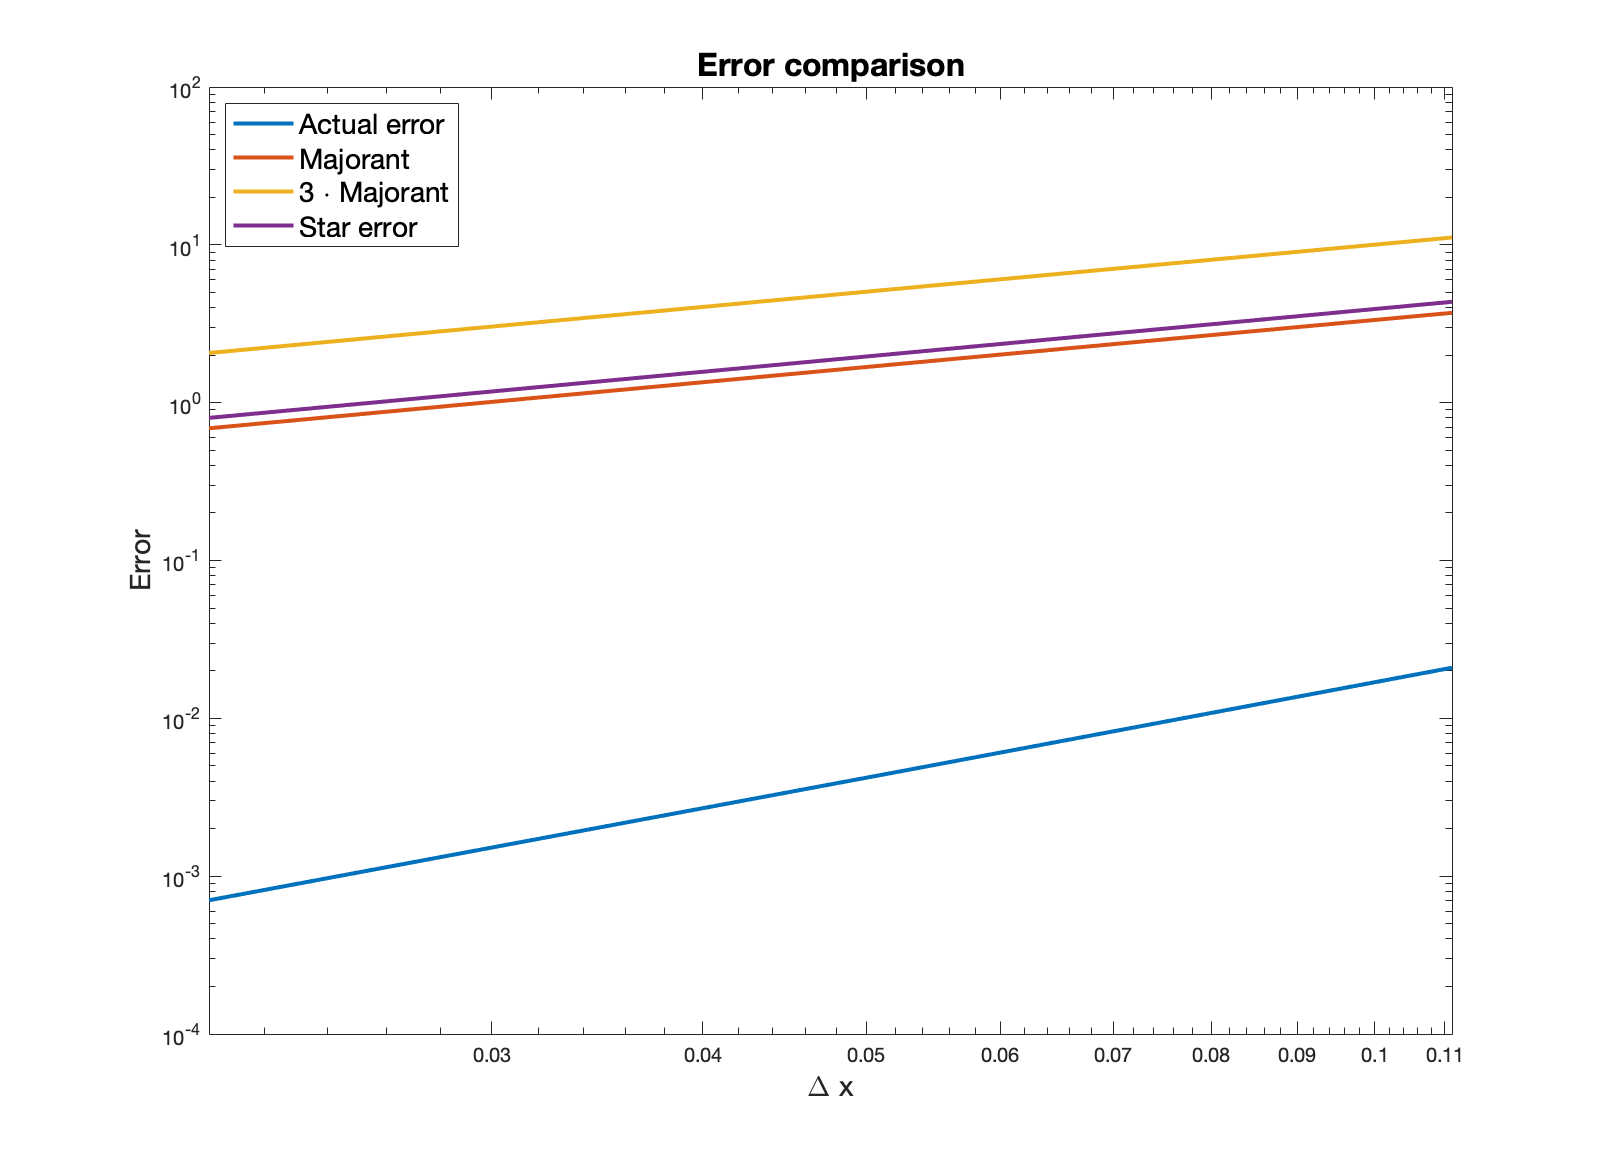
\includegraphics[scale=0.18]{errors}
        \end{figure}
    \end{frame}
\end{document}